\chapter{SYCL implementation of CLUE}
\label{ch:3}
\section{Porting the standalone version of CLUE}
\subsection{Notable changes}
As previously discussed, the first step in the porting experience was the translation of CLUE in SYCL. The original code, found on a CMS Patatrack gitlab repository \cite{clue_repo}, already implemented the CPU serial, the CUDA and the multithreaded CPU versions (the latter using Threading Building Blocks\footnote{Threading Building Blocks (TBB) is a performance library that allows to simplify the work of adding parallelism to complex applications across different architectures \cite{TBB}.}). 

Since, as highlighted above, oneAPI provides the developers with a conversion tool from CUDA code to SYCL, the conversion work begun by passing the CUDA version's code through the tool. This produced a non-working SYCL code output which had to be modified and adjusted. While the underling logic and implementations are almost exactly the same, two examples of practical differences between the CUDA implementation and the SYCL one are explored in the following: 
\begin{itemize}
    \item kernel submission;
    \item use of variables inside kernels as demonstrated in section~\ref{ch:kernels_execution}
\end{itemize}
\subsubsection{CLUE Kernel submission CUDA vs SYCL}
CLUE is split into five kernels each of which deals with one part of the clustering procedure, as highlighted in section~\ref{ch:clustering_procedure}. In CUDA, work in divided in a grid-block-thread fashion. This means that when a kernel is submitted, the whole problem is covered by the grid size, then it's split in smaller parts each of which is assigned to a block that finally assigns a single task to each of its threads. SYCL work division, while similar in principle, is quite different to work with since it needs to adapt to a multitude of heterogeneous backends. SYCL work division can be mapped to the CUDA one almost exactly in case the code is running on a GPU. In particular, the CUDA hierarchy \Verb "grid-block-thread" becomes \Verb "nd_range-work-group-work-item" in SYCL. It must be stressed that this mapping concerns only GPUs, while on CPUs the hardware mapping can look quite different depending on the vectorization\footnote{Automatic compiler optimization which processes an operation on multiple pair of operands at the same time. Compilers can generally transform \Verb "for" loops in a set of vector operations} capabilities of the specific device.
In code~\ref{code:kernel_submission} the two equivalent ways to cover the same problem with the same work division in CUDA and SYCL are shown.

\begin{figure}[ht!]
\renewcommand{\figurename}{Code}
\begin{minted}[linenos]{cpp}
// CUDA version
const dim3 blockSize(numThreadsPerBlock, 1, 1);
const dim3 gridSize(numBlocks, 1, 1);
 
kernel<<<gridSize, blockSize>>>(d_input, d_output);

// SYCL version
auto queue = sycl::queue(sycl::default_selector{});
const sycl::range<3> blockSize(1, 1,numThreadsPerBlock);
const sycl::range<3> gridSize(1, 1, numBlocks);

queue.submit([&](sycl::handler& cgh) 
{
  cgh.parallel_for(sycl::nd_range<3>(gridSize * blockSize, blockSize), 
                                     [=](sycl::nd_item<3> item)
    {
        kernel(d_input, d_output, item);
    });
});
}
\end{minted}
\caption{Difference in work division and kernel submission in CUDA and SYCL.}
\label{code:kernel_submission}
\end{figure}

One thing to note in the example above is the difference in the order of dimensions between CUDA \Verb "dim3" and \Verb "sycl::range". In fact, the former follows the order (x, y, z), while the latter follows the inverted order (z, y, x). While this might not be an issue in general, specifically when running SYCL code on NVIDIA GPUs, the order of the dimensions become relevant as most of those GPUs have limited thread capabilities on the z dimension. For example on the NVIDIA A10 used for testing, the z dimension of \Verb "blockSize" is limited to a maximum of 64, while the other dimensions can go up to 1024.
These considerations has led us to submit kernels in the way demonstrated above to keep the mapping of one point per thread in the clustering procedure independently by the hardware that would actually run the code through SYCL. 

\subsection{Physics validation and performance comparison}
In order to validate the physics results of the new implementation, a set of synthetic datasets, previously already used to validate the physics results of CLUE, was considered. In this case, the outputs produced by the different implementations were compared while using the same input data and parameters to demote outliers. As described in section~\ref{ch:clustering_procedure}, points with density below the critical one could be demoted to outliers if their $\delta$ is larger than the specified threshold. The specific synthetic dataset used was generated in such a way to resemble high-occupancy events with conditions similar to what it is expected in the proposed high granularity calorimeter upgrade for CMS. Results were validated in different scenarios, each time increasing the number of hits per event. In particular, a total of 100 layers are input to CLUE simultaneously, with each layer having a fixed number of points with a unit weight in such a way that the density represents clusters whose energy distribution follows a Gaussian centered in the middle of the cluster with standard deviation $\sigma$ set to 3 cm. 5\% of the points are generated as noise distributed uniformly over the layers. To test CLUE's performance scaling, the number of points in each layer is increased from 1,000 to 10,000 in 10 equaling steps so that the total number of points per event in the test ranges between $10^5$ and $10^6$. In figure~\ref{fig:clue_standalone_cpu} is shown the performance scaling of the different CPU implementations. The results of these comparisons are obtained as the mean timing of ten runs of the algorithm. Note that SYCL seems to provide a massive advantage compared to native serial code when running on the same hardware. This is mostly due to its native support for multithreading to oneTBB, the oneAPI implementations of Threading Building Blocks. While the serial code is inherently limited to only use one CPU thread, the SYCL version can offload work to all of the available threads. The other TBB implementation seen in the graph shows as a sort of in-between in terms of performance. This behaviour can be explained by the particular version of TBB used to implement CLUE. In particular the standalone version of CLUE uses Alpaka to implement TBB and, at the time of the data taking, this version of TBB had thread locks that decreased performance significantly due to the implementation of atomic operations in Alpaka. This performance issue should be solved in later releases to bring the performance more in line with the one demonstrated by SYCL. In any case, a part from an outlier in the TBB implementation probably due to the overhead of creating many threads compared to the execution of a simple task, the performance scales linearly with the number of points per layer as per expectations.

\begin{figure}[H]
    \centering
    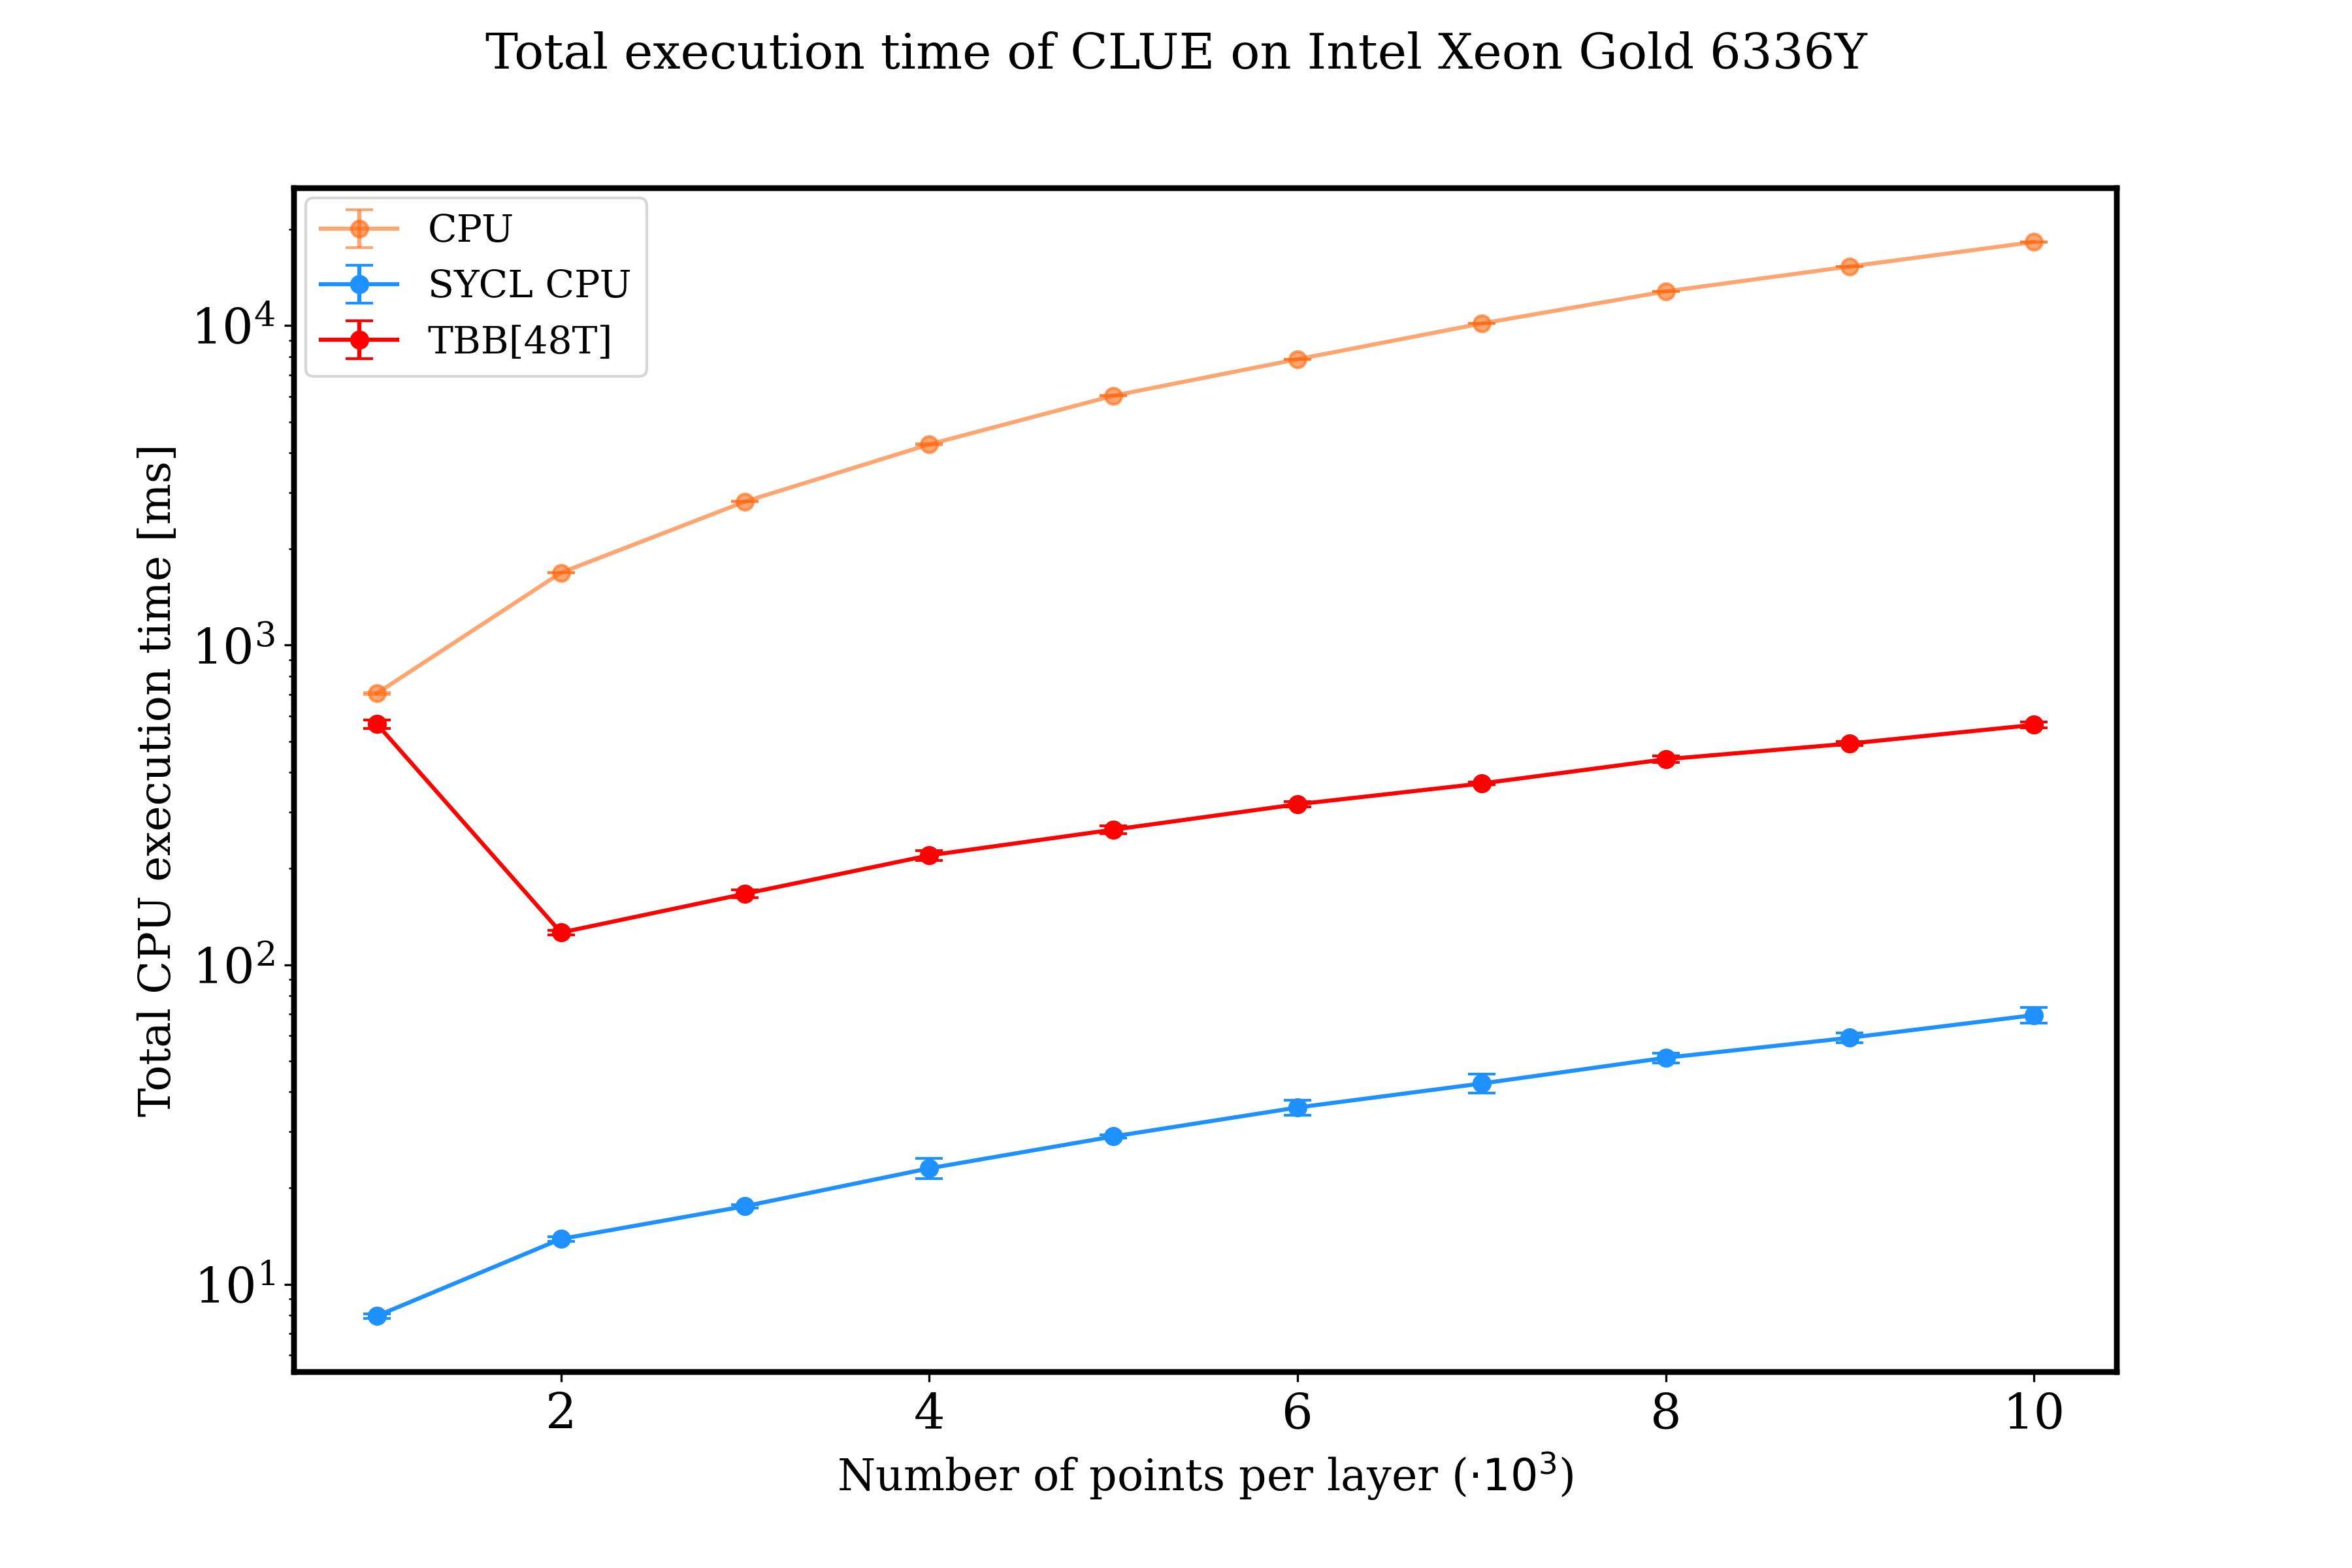
\includegraphics[width=\textwidth]{media/clue_standalone_cpu.png}
    \caption{Performance comparison of CLUE's different CPU implementations. Note that the y axis is in log scale, showing the massive improvement that SYCL has over the native serial code. This advantage is mostly given by the native support for multithreading in SYCL applications.}
    \label{fig:clue_standalone_cpu}
\end{figure}

However, the greatest speedup in execution time is achieved when using GPUs. The main aim of the porting was to show that it is possible to write a single source code to then compile and run on a multitude of devices. In figure~\ref{fig:clue_standalone_cuda} it is shown how the total execution time of CLUE running on the same GPU is almost the same when using SYCL through the CUDA backend with respect to native CUDA code. The SYCL code is completely unchanged compared to the CPU version shown above, thus achieving at least one of the objectives of heterogeneous computing. The only difference between this executable and the one used for the CPU benchmarking is the compiler used to produce it. In fact, oneAPI's compiler, dpcpp, does not yet support the CUDA backend natively so, while its integration is in development, the open source fork of dpcpp, LLVM, was used to compile the project and test it on NVIDIA hardware. Especially considering that this backend is not officially supported yet, the results look extremely promising.

\begin{figure}[H]
    \centering
    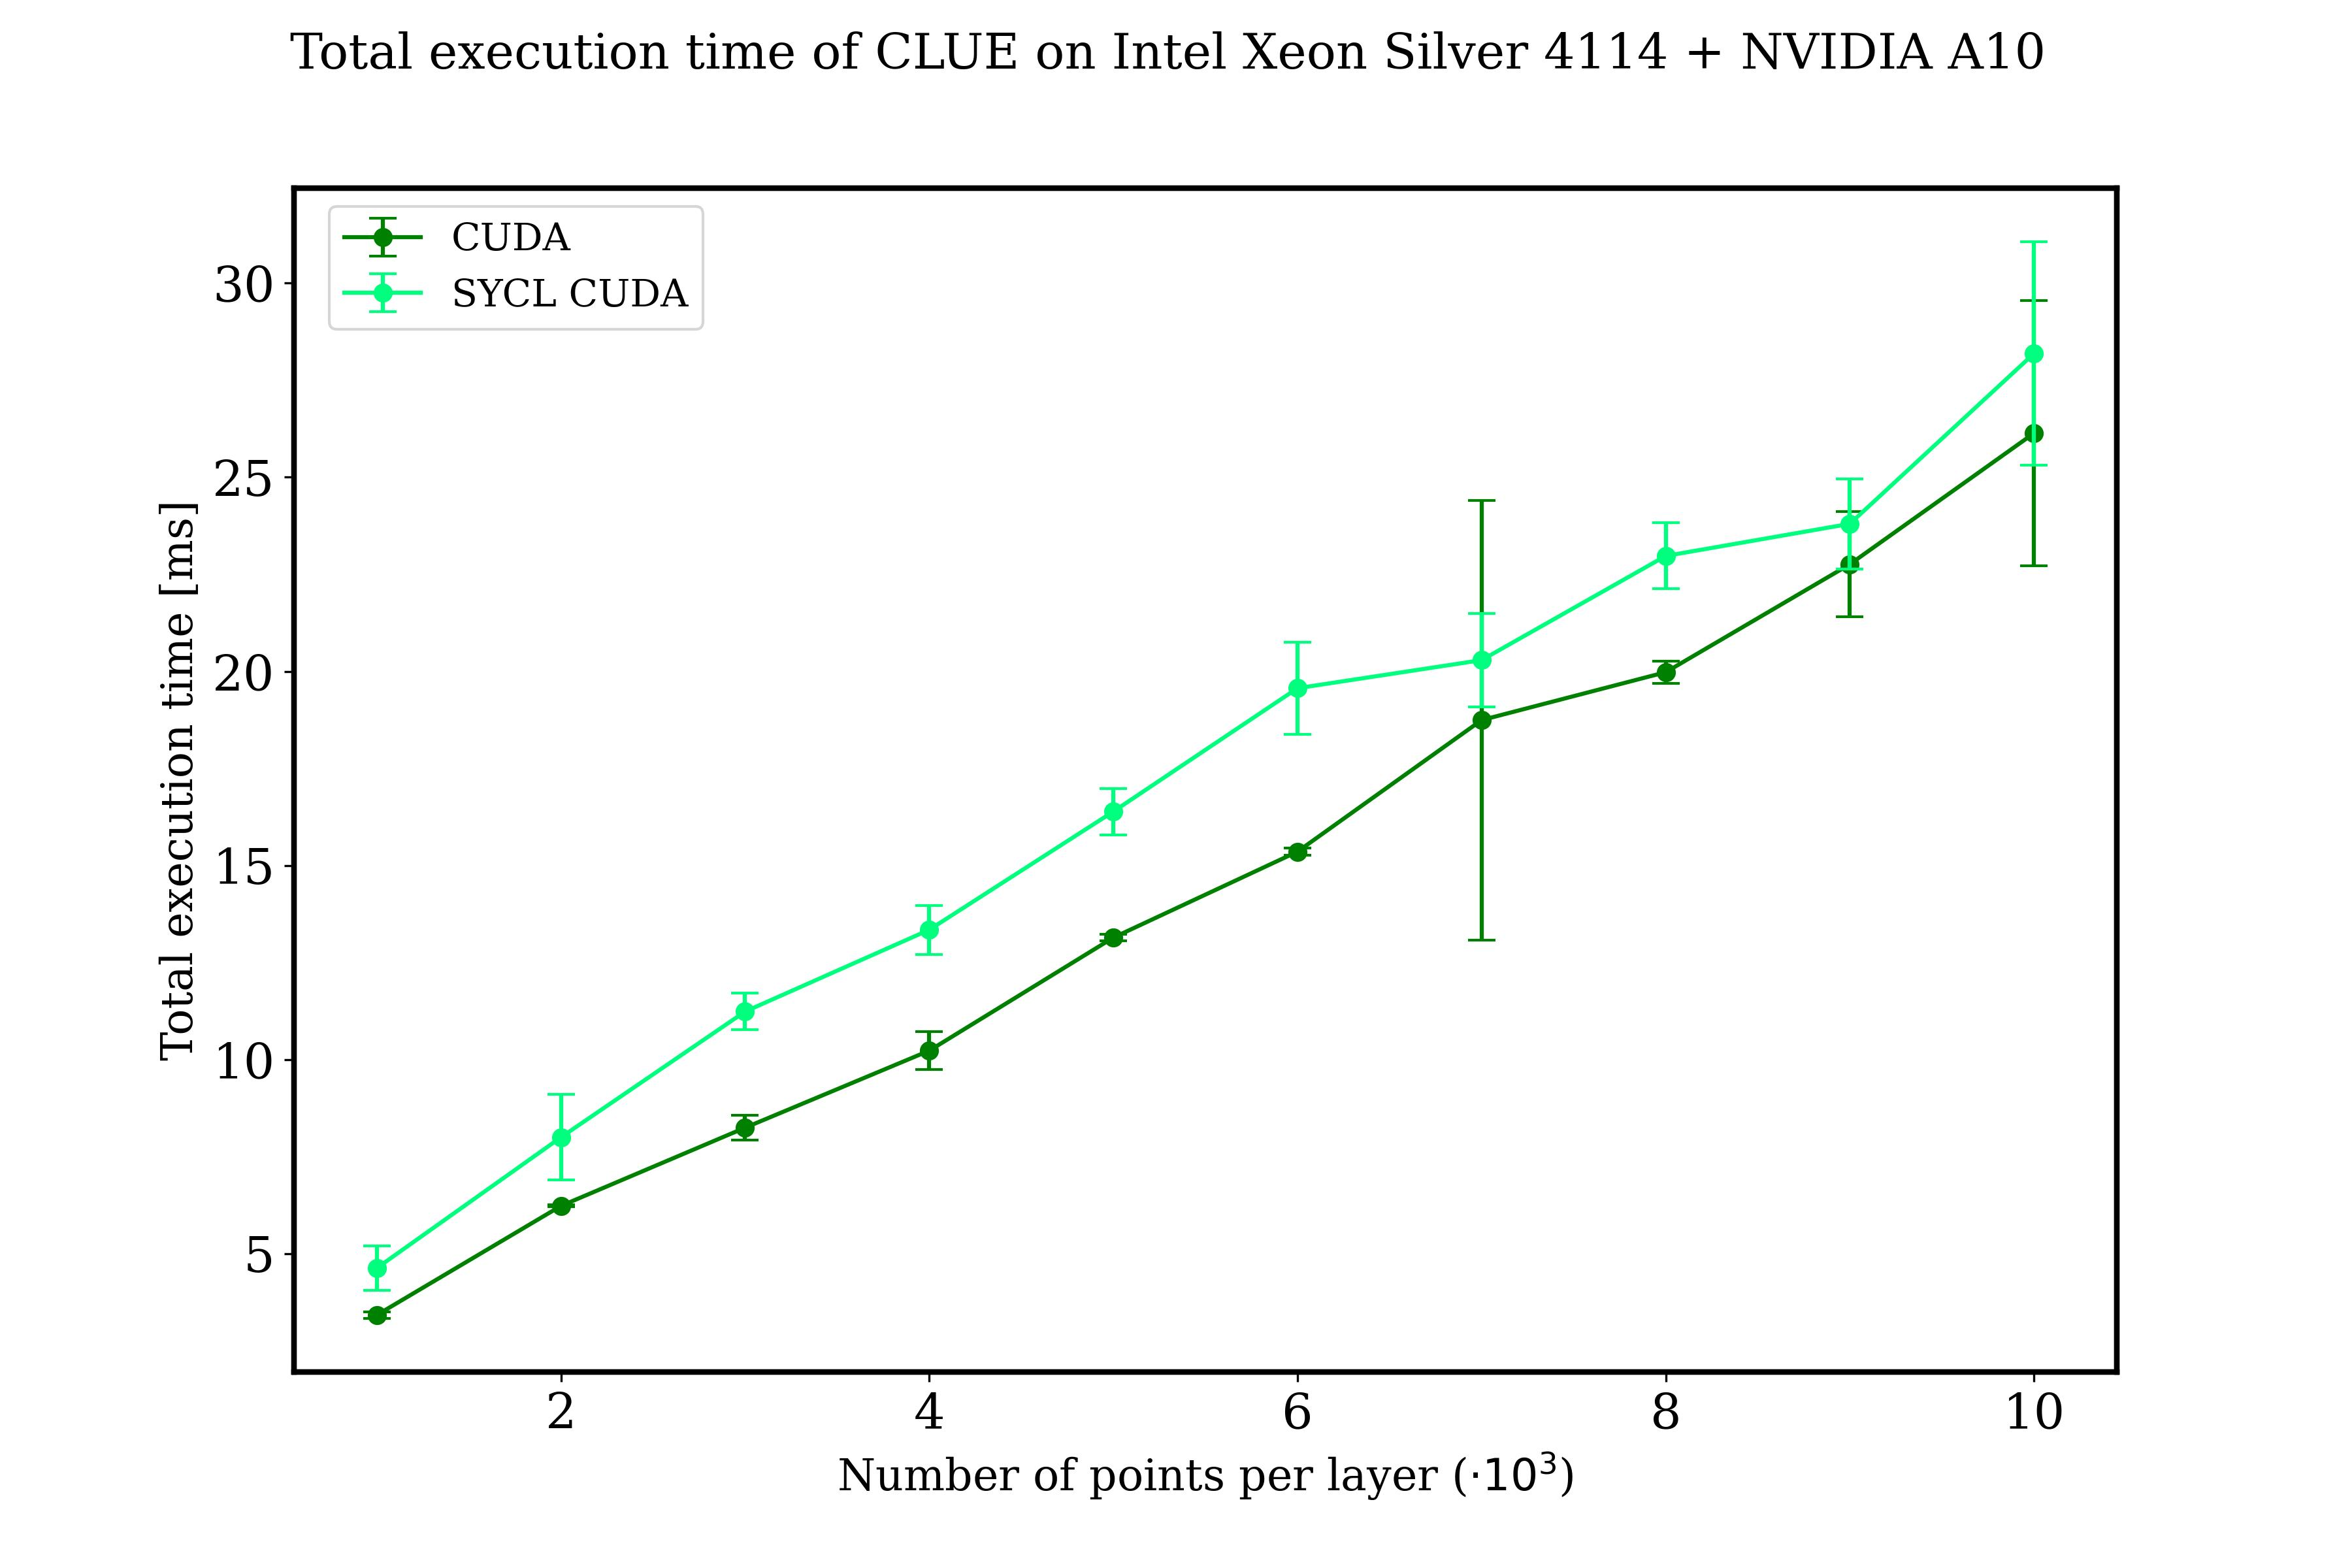
\includegraphics[width=\textwidth]{media/clue_standalone_cuda.jpg}
    \caption{Performance comparison between native CUDA code and SYCL code running through the CUDA backend.}
    \label{fig:clue_standalone_cuda}
\end{figure}

Note that, in general, using GPUs allows to improve the performance by roughly 3 times even when compared to multithreaded execution on CPU and the increase is even more noticeable with respect to all the others implementations.

\section{Integrating CLUE in a CMSSW-like framework}
As previously stated, the standalone port was carried out mainly to experiment with SYCL and become familiar with its functioning. Once such task was completed, actual physics evaluation and performance measurements had to be carried out in a framework resembling the one used for general event reconstruction: CMSSW. This required significant changes and adaptations as well as actual developments on the framework itself, but allowed us to obtain way better results all both in terms of raw performance and in terms of physics reconstruction.

\subsection{An introduction to the framework}
Before getting to the framework-integrated and improved version of CLUE, let us introduce the basics of that framework. Similarly to what has previously been done by the Patatrack CMS group for their standalone pixel tracking module \cite{pixeltrack}, a crude approximation of CMSSW's framework \cite{cmssw} was used to process data and schedule the execution of CLUE. 

The framework's main goal is to facilitate the deployment of software. The core of the execution is given by the Event Data Model (EDM) which is centered around the concept of an \emph{Event}. Topologically, an Event is a C++ object which contains all of the raw data and information related to a particular collision. In the specific case of clue, one Event contains the 2D coordinates, layer and energy of each hit related to a single collision. The Event is used to pass data from one module to the next and it represents the only way to access or modify data. Some modules might require additional information to process events which is provided to them through the relevant \emph{Event Setup} module. Moreover, the framework is modular, meaning that each step of the reconstruction is represented by a separate plugin that can be plugged in the main run. Plugins are compiled in shared libraries and the execution must be configured to schedule and run the desired plugins. While the framework allows for six different types of modules  only the types used in CLUE are explained as to not shift the focus of our discussions:
\begin{itemize}
    \item Source: Reads in  an Event from an input file (csv, binary, ROOT...), gives the Event status information and can add data on host memory. 
    \item EDProducer: Producer modules read in data from the Event in one format, produce something from the data and emplace the output, in a different format, back into the Event.
    \item OutputModule: Reads data from the Event and stores the output to external media.
\end{itemize}

In this context, it is possible to offload part of the workload to be executed on heterogeneous devices when using one of the implementations of the framework and modules that take advantage of a compatibility layer such as Alpaka or SYCL.

To exemplify the concepts described above, in figure~\ref{fig:hclue_workflow} the steps executed by CLUE when integrated in the framework are shown. Modules are grouped by color and the workflow follows a top to bottom order following the arrows direction. The red module is a future, to be developed, integration with the 3D clustering module used in CMSSW's reconstruction. ESProducers are not pictured as not to clutter the workflow, but each module, a part from the Source, has an associated one of the aforementioned type that feeds it relevant input data, like the parameters to use for the clustering. 

\begin{figure}[H]
    \centering
    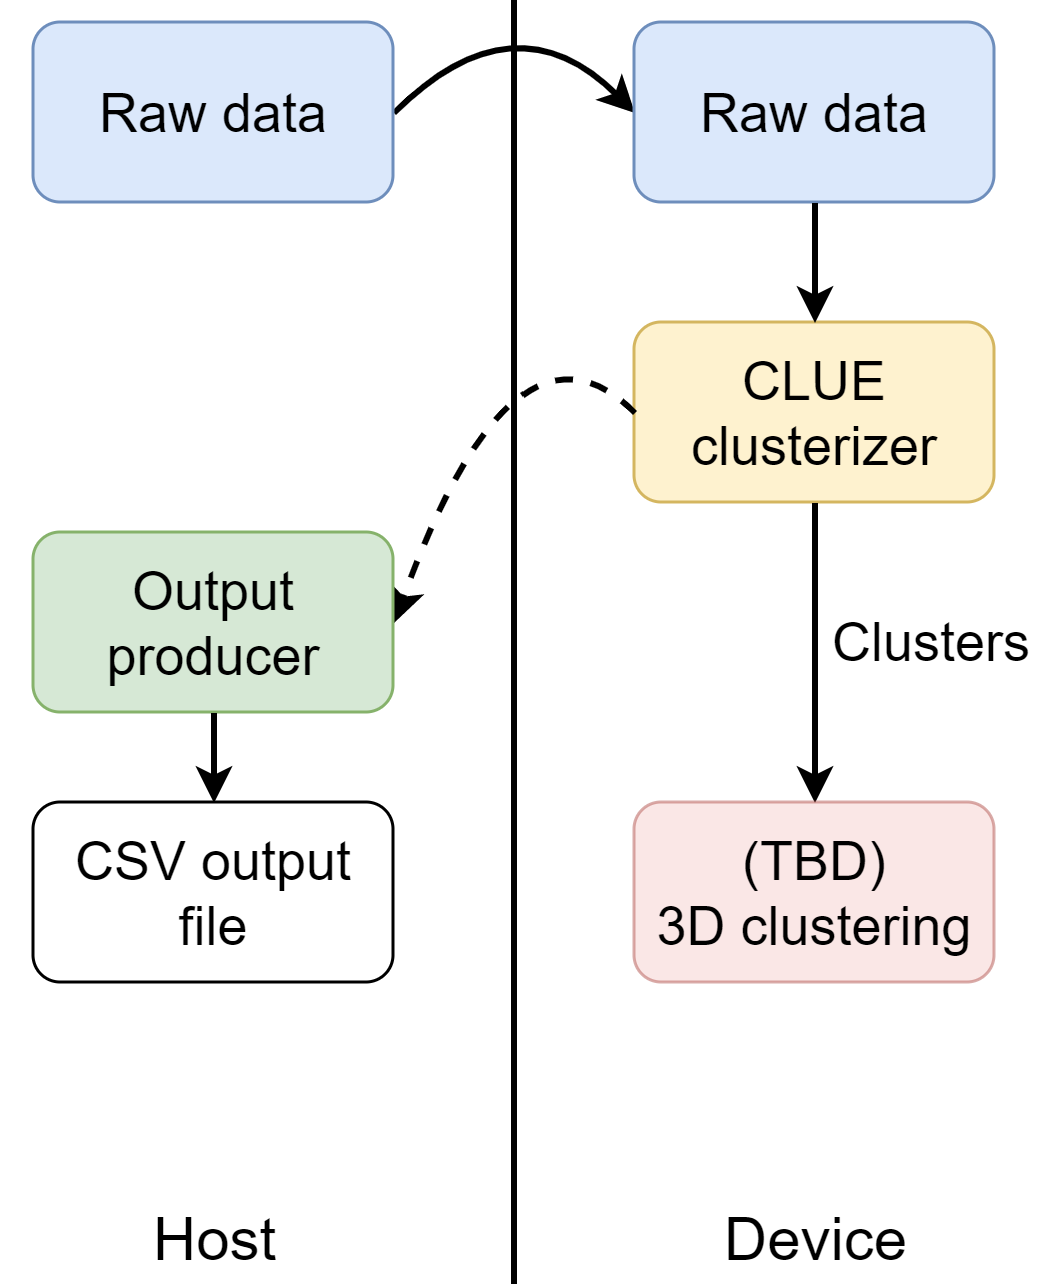
\includegraphics[scale=0.7]{media/hclue_workflow.png}
    \caption{CLUE workflow inside a CMSSW-like framework. Blue modules are results of Source, the yellow module is the single EDProducer, while the green module is the OutputModule which (optionally) produces a csv output file per event at the end.}
    \label{fig:hclue_workflow}
\end{figure}

Another fundamental aspect of the framework is its integration with Threading Building Blocks to take advantage of multiple threads and execute more events at the same time. This last aspect, in particular is carried out by creating multiple \Verb "EDM streams". Each one of these \emph{streams} correspond to executing the whole program, in our case the clustering, on a different event and the framework allows the creation and execution of multiple streams at the same time. This means that on a more capable device, like a multithreaded CPU or a GPU, multiple events can be analyzed at the same time, thus greatly improving the total throughput (number of events processed per second) of the algorithm.
CLUE hence acts as a somewhat simple introduction to the framework's inner workings and provides a benchmarking platform for the different implementations. One final thing to note is that by detaching modules from CMSSW to integrate them into standalone versions of the framework allows to experiment way more freely while also testing performance before integrating wider changes into CMSSW's code base, this idea led to the creation to the standalone pixel tracking module as well as this CLUE implementation.

\subsection{Changes and improvements from the standalone version}
Integrating CLUE in the framework allows to take advantage of more advanced scheduling, finer control on the number of threads and concurrent streams used for the execution while also providing better performance measuring capabilities. However, in order to fully take advantage of the framework, significant changes had to be made to the core of its SYCL implementation. 

Starting from the most fundamental aspect, some parts of the framework, ported from CUDA, needed to be optimized for SYCL inner workings, while some others had to be rewritten entirely. First up, since SYCL is designed to be compatible with multiple backends its device selection logic is different from the one seen in CUDA and more akin to alpaka. In the current version of the code, the user can select which device to offload work to by a simple command line parameter \Verb "--device" followed by the kind of device wanted or its backend. The device selector will take care of finding all of the compatible devices and offload work to the selected one by creating an in-order queue on that device per \Verb "EDM stream" to schedule memory operations and kernels execution.

When offloading work to an accelerator, the most costly operation in terms of overhead is device memory allocation. That is why the framework includes a module for caching the allocations, which had to be entirely rewritten for its SYCL implementation. This modules makes it so that the least amount of allocations is executed and that memory that has been freed can be reused without needing another allocation. Using CLUE as an example, the algorithm needs 13 allocations per run for the input variables, the results and some inner variables used to make calculations. Using the caching allocator, when running with a single stream, CLUE will allocate 13 blocks of the required size in the device memory, then reuse those blocks for every event and deallocate them, thus freeing the device memory, at the end of the execution. At the beginning of the execution one caching allocator is constructed on each available device. Device memory is accessed though custom-defined unique pointers which interface directly with the caching allocator on the specific device. This approach has two main benefits:
\begin{itemize}
    \item Costly device memory allocations are reduced to a minimum by reusing memory whenever possible;
    \item All of the cached memory is freed at the end of the execution, thus allowing no memory leaks.
\end{itemize}

From the algorithm's point of view, this changes mainly reflect in where the allocations can take place. Since a single \Verb "sycl::queue" is produced per event and gets propagated by the framework and the queue is needed for all of the memory operations and kernels scheduling, the algorithm had to be tweaked to perform queue-bound operations when one is obtainable from the \Verb "EDM event".

\section{Results}
The framework-integrated version of CLUE, from here on referred to as heterogeneous CLUE, was tested against a simulated dataset obtained by running the reconstruction of a ttbar event with 200 pileup, on a recent version of CMMSW and dumping the information of hits to a binary file. The conditions chosen are the most similar to the ones that would be seen in the proposed HGCAL upgrade \cite{hgcal}.
\subsection{Physics performance}
Heterogeneous CLUE's performance have been evaluated on both CPUs and GPUs with different backends using Alpaka, SYCL and native code whenever possible. In particular, the following hardware was used to benchmark the algorithm:

\begin{itemize}
    \item Intel(R) Xeon(R) Silver 4114 CPU 2.20GHz with driver OpenCL \newline [2022.14.7.0.30\textunderscore160000];
    \item NVIDIA Tesla T4 with driver CUDA [11.6];
    \item Unreleased Intel GPU;
\end{itemize} 

Starting from the worst performers, in figure~\ref{fig:hclue_cpu_performance} is shown the performance scaling with the number of threads of heterogeneous CLUE running on CPU. As seen in the standalone version, the SYCL implementations looks to be able to take better advantage of multithreading on CPU showing a 21-57 \% performance increase when compared to Alpaka and 14-102\% improvement with respect to the native serial implementation. The measurements are the mean of 10 consecutive runs on 1000 events. The exact results are shown in table~\ref{tab:hclue_cpu_performance}. One particular case that deserves to be highlighted is the single-thread one. Both Alpaka and the native implementations show less than half the performance of SYCL in this case. This happens because SYCL is actually using two threads in this particular instance by relying on the multithreading capabilities of the CPU and dedicating one thread to the framework execution and one to the algorithm itself. This is even more evident noting that the throughput remains almost exactly the same when using two threads.

\begin{figure}[H]
    \centering
    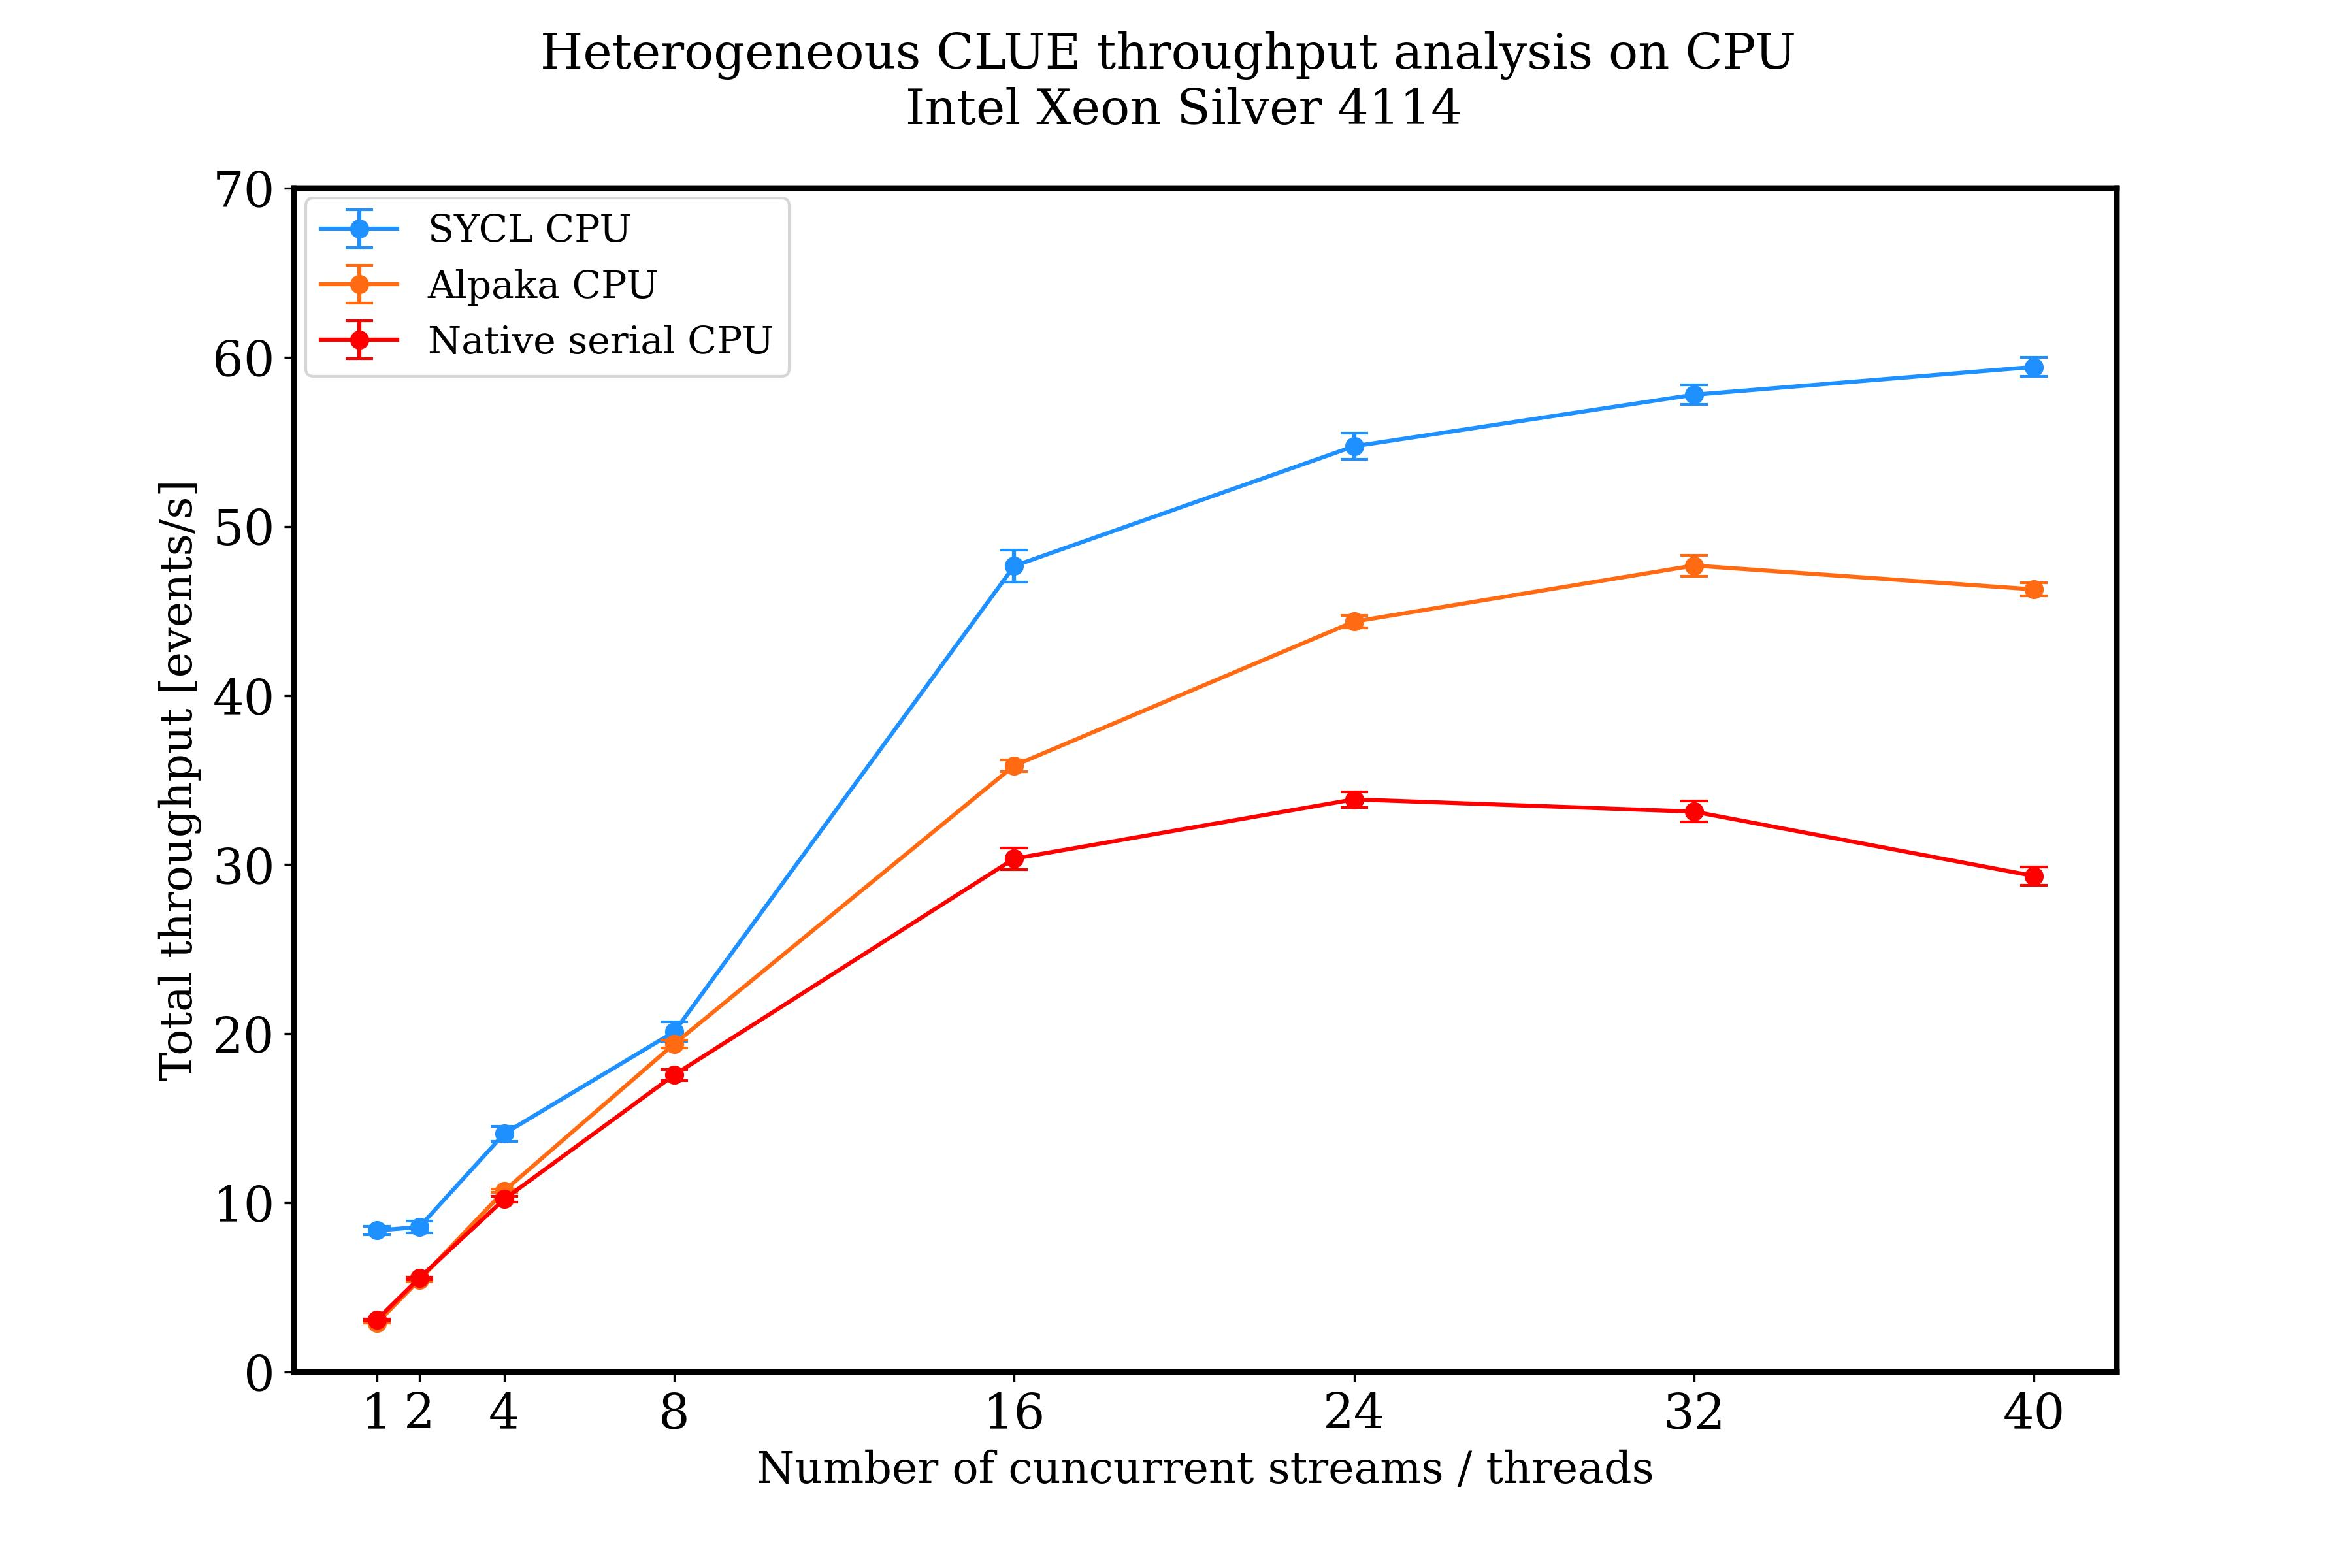
\includegraphics[width=\textwidth]{media/hclue_cpu_performance.jpg}
    \caption{Performance comparison of the different CPU implementations of CLUE.}
    \label{fig:hclue_cpu_performance}
\end{figure}

\begin{table}[htb]
    \centering
    \begin{tabular}{|c|c|c|c|}
 \hline
 \multicolumn{4}{|c|}{Total throughput on Intel Xeon Silver 4114 (ev/s)} \\
 \hline
 Threads & Alpaka & Native serial & SYCL\\
 \hline
 1 & 2.894 $\pm$ 0.014 & 3.09 $\pm$ 0.05 & 8.4 $\pm$ 0.3 \\
 2 & 5.44 $\pm$ 0.12 & 5.55 $\pm$ 0.05 & 8.6 $\pm$	0.3 \\
 4 & 10.72 $\pm$ 0.09 &	10.22 $\pm$	0.15 & 14.1 $\pm$ 0.4 \\
 8 & 19.4 $\pm$ 0.2 & 17.6 $\pm$ 0.3 & 20.1 $\pm$ 0.6 \\
 16 & 35.9 $\pm$ 0.4 & 30.4 $\pm$ 0.6 & 47.7 $\pm$ 0.9 \\
 24	& 44.4 $\pm$ 0.4 & 33.9 $\pm$ 0.5 & 54.7 $\pm$ 0.8 \\
 32	& 47.7 $\pm$ 0.6 & 33.1 $\pm$ 0.6 & 57.8 $\pm$ 0.6 \\
 40	& 46.2 $\pm$ 0.4	& 29.3 $\pm$ 0.5	& 59.4 $\pm$ 0.6 \\
 \hline
\end{tabular}
    \caption{Detailed throughput analysis for the CPU implementations of heterogeneous CLUE.}
    \label{tab:hclue_cpu_performance}
\end{table}

Moving to the GPU implementations, the throughput increases from 3 to 10 times depending on the comparisons. In figure~\ref{fig:hclue_cuda_performance} is shown the comparisons between the two different compatibility layers discussed, executing logically identical code on the same hardware.

\begin{figure}[H]
    \centering
    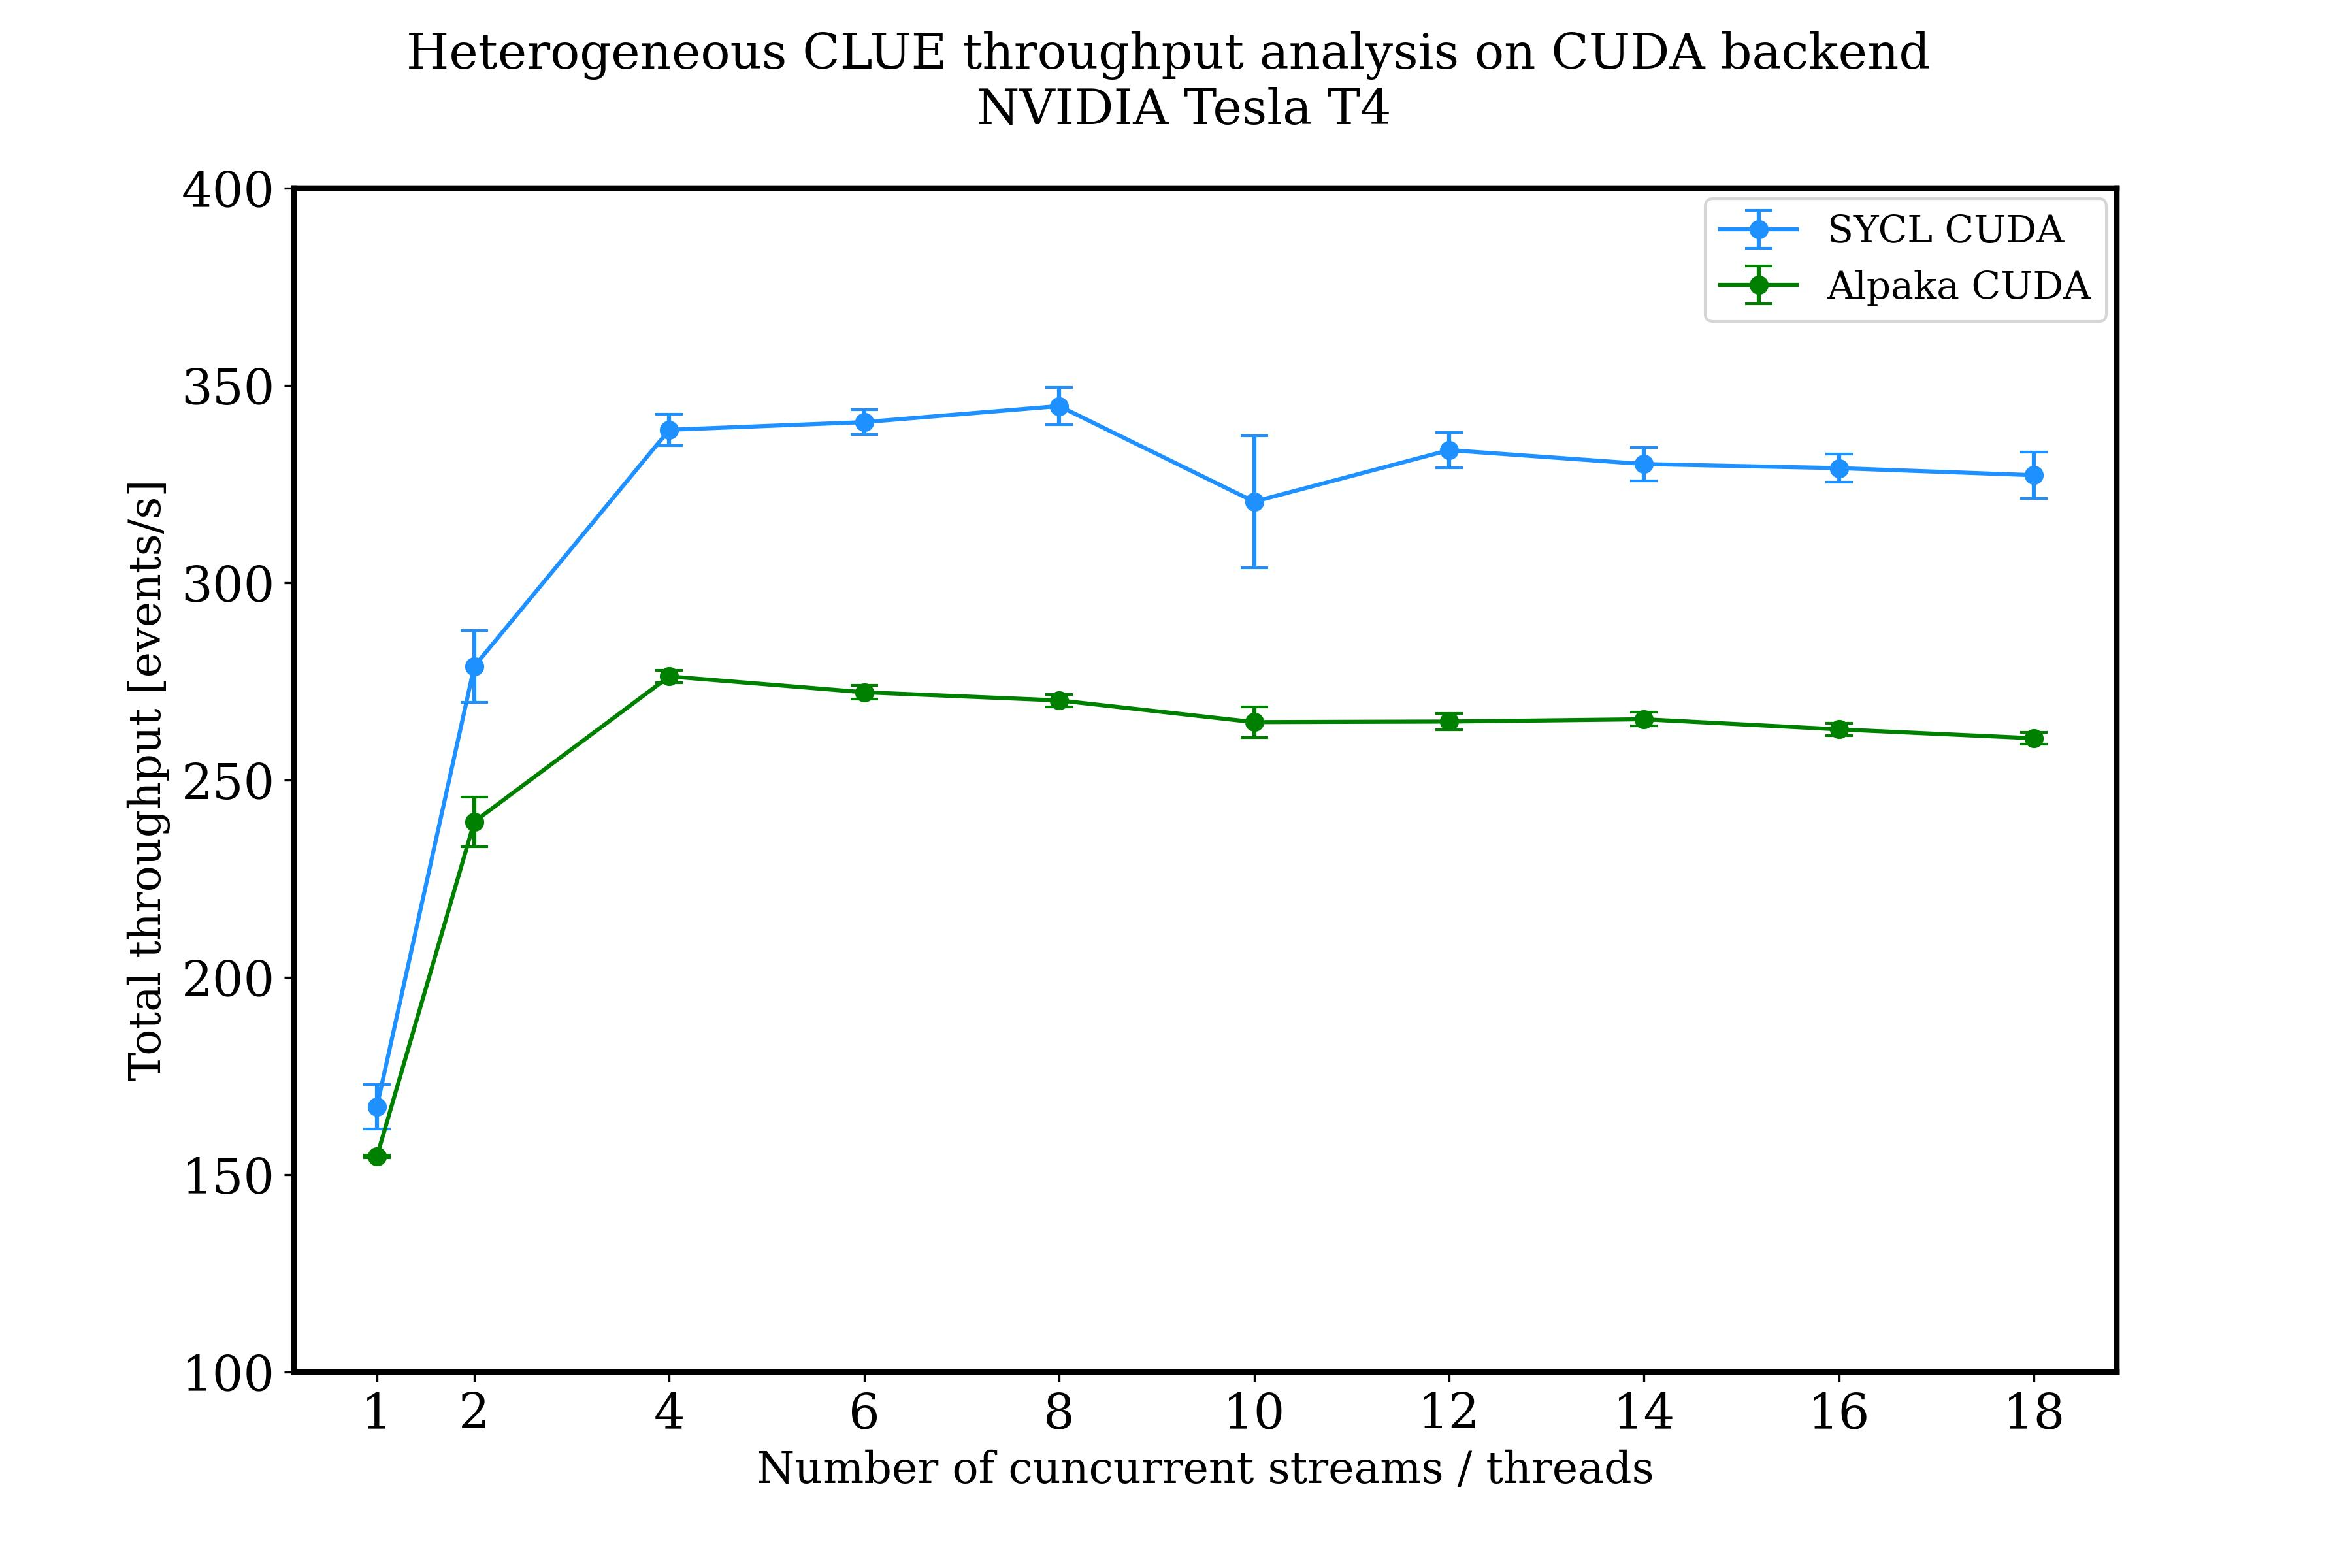
\includegraphics[width=\textwidth]{media/hclue_cuda_performance.jpg}
    \caption{Comparison of SYCL and Alpaka CLUE implementations when running on the CUDA backend}
    \label{fig:hclue_cuda_performance}
\end{figure}
\noindent
The performance difference is trickier to explain in this case, but on a general level it looks like that, at least for this particular workload and hardware, SYCL has better memory management capabilities than Alpaka, thus improving speed when transferring data, allocating and setting memory and synchronizing streams. One thing to note is that the increasing number of streams can lead to performance degradation and instability, especially on SYCL, which shows its best performance when using 6 threads / streams. A detailed breakdown of the data is presented in table~\ref{tab:hclue_cuda_performance}.

\begin{table}[H]
    \centering
    \begin{tabular}{|c|c|c|}
 \hline
 \multicolumn{3}{|c|}{Total throughput on NVIDIA Tesla T4 (ev/s)} \\
 \hline
 Streams & Alpaka & SYCL\\
 \hline
 1 & 154.6 $\pm$ 0.3 & 167 $\pm$ 6 \\
 2 & 239 $\pm$ 6 & 279 $\pm$ 9 \\
 4 & 277 $\pm$ 2 &	339 $\pm$ 4 \\
 6 & 272 $\pm$ 2 & 341 $\pm$ 3 \\
 8 & 270 $\pm$ 2 & 345 $\pm$ 5 \\
 10 & 265 $\pm$	4 &	321 $\pm$ 17 \\
 12 & 265 $\pm$ 2 & 334 $\pm$ 4 \\
 14 & 265 $\pm$ 2 & 330 $\pm$ 4 \\
 16 & 262 $\pm$	2 &	329 $\pm$ 4 \\
 18 & 261 $\pm$ 2 &	327 $\pm$ 6 \\
 \hline
\end{tabular}
    \caption{Detailed throughput analysis for the CUDA implementations of heterogeneous CLUE.}
    \label{tab:hclue_cuda_performance}
\end{table}

Finally, throughput analysis on the unreleased Intel GPU cannot be disclosed due to the pre-alpha state of the hardware, which is still under NDA. However, testing on this hardware has been successful in showing that a single SYCL source code can run on CPUs, Intel GPUs and NVIDIA GPUs. This demonstrates the potential of SYCL as a portability layer to ease code maintainability across different backends.

\subsection{Porting considerations}
As discussed throughout this thesis, multiple adjustments had to be made in order to transition from CUDA to SYCL. In this context, the compatibility tool developed by Intel has provided help on more than one occasion, but its output cannot yet be trusted on all the situations, especially when dealing with more complex projects. In particular, some of the areas in which the tool provides little to no help are:
\begin{itemize}
    \item Porting of more complex projects, made up of multiple compilation units;
    \item Error management;
    \item Atomic operations.
\end{itemize}

Regarding the second point, the error management system employed by SYCL is based on throwing and caching exceptions, similarly to what is done in plain C++, while CUDA implements its own error management system. Because of this, it is up to the programmer to add the relevant checks to make sure that the SYCL code can handle eventual errors. As far as atomic operations\footnote{In programming, an atomic operation guarantees exclusive access to a particular memory address to the thread that is executing the operation itself.} are concerned, SYCL implementation is still pretty much undocumented and lacks some fundamental CUDA methods. Re-implementing needed methods is possible, but must be done on a case-by-case basis and completely by hand. 

In general, expressing parallelism through SYCL is more difficult than doing the same through CUDA, mostly due to the heterogeneous nature of SYCL code. The creation of \Verb "nd_ranges" with the desired dimensions to cover any specific problem is extremely verbose and the methods to obtain the compute capabilities of the device in use are not always helpfule in creating an optimized work division. This problem becomes especially evident in complex code that makes extensive use of CUDA warps\footnote{In CUDA, a warp is a collection of 32 threads that execute the same instruction.} which are inherently more difficult to port to other backends. One possible solution is given by utilizing sub-groups in SYCL, though sub-group dimension is hardware-dependent and needs to be known at compile time in the kernel invocation.